%--
\chapter{图遍历 (L10)}


%----------------------------------------
\section*{授课提纲}

\nid 图算法总览（\S\ref{sec:graph-overview}）：
%--
\begin{itemize}
    \item 图算法问题：从\ul{遍历}到\ul{优化}；
    \item 图算法策略：从\ul{贪心}到\ul{动态规划}。
\end{itemize}

\nid 框架的基本概念：
%--
\begin{itemize}
    \item 共性内容的固化；
    \item 具体内容的细化：参数化、定制化。
\end{itemize}


\nid 精化（层层细化）观点下的图遍历：
%--
\begin{itemize}
    \item 不变式的概念（回顾）、精化的概念；
    \item 抽象的WFS框架（\S \ref{sec:wfs}）；
    \item WFS $\Rightarrow$ DFS、BFS、\alg{BestFS}。
\end{itemize}


\nid DFS框架基础：
%--
\begin{itemize}
    \item 抽象DFS框架；
    \item 嵌入application-specific处理的3组（共5个）时机。
\end{itemize}

\nid DFS框架的增强：
%--
\begin{itemize}
    \item 点着色：W $\Rightarrow$ G $\Rightarrow$ B；
    \item 边着色：TE、BE、DE、CE；
    \item 时间的引入：\textsc{StartTime}、\textsc{FinishTime}、\textsc{ActiveInterval}。
\end{itemize}

%----------------------------------------
\section{图算法总览} \label{sec:graph-overview}

首先我们列出图算法部分的关键知识点，如图\ref{fig:graph-overview}所示。然后我们从问题和策略两个正交的维度，来鸟瞰这些知识点。

%--
\begin{figure}[htbp]
    \center
    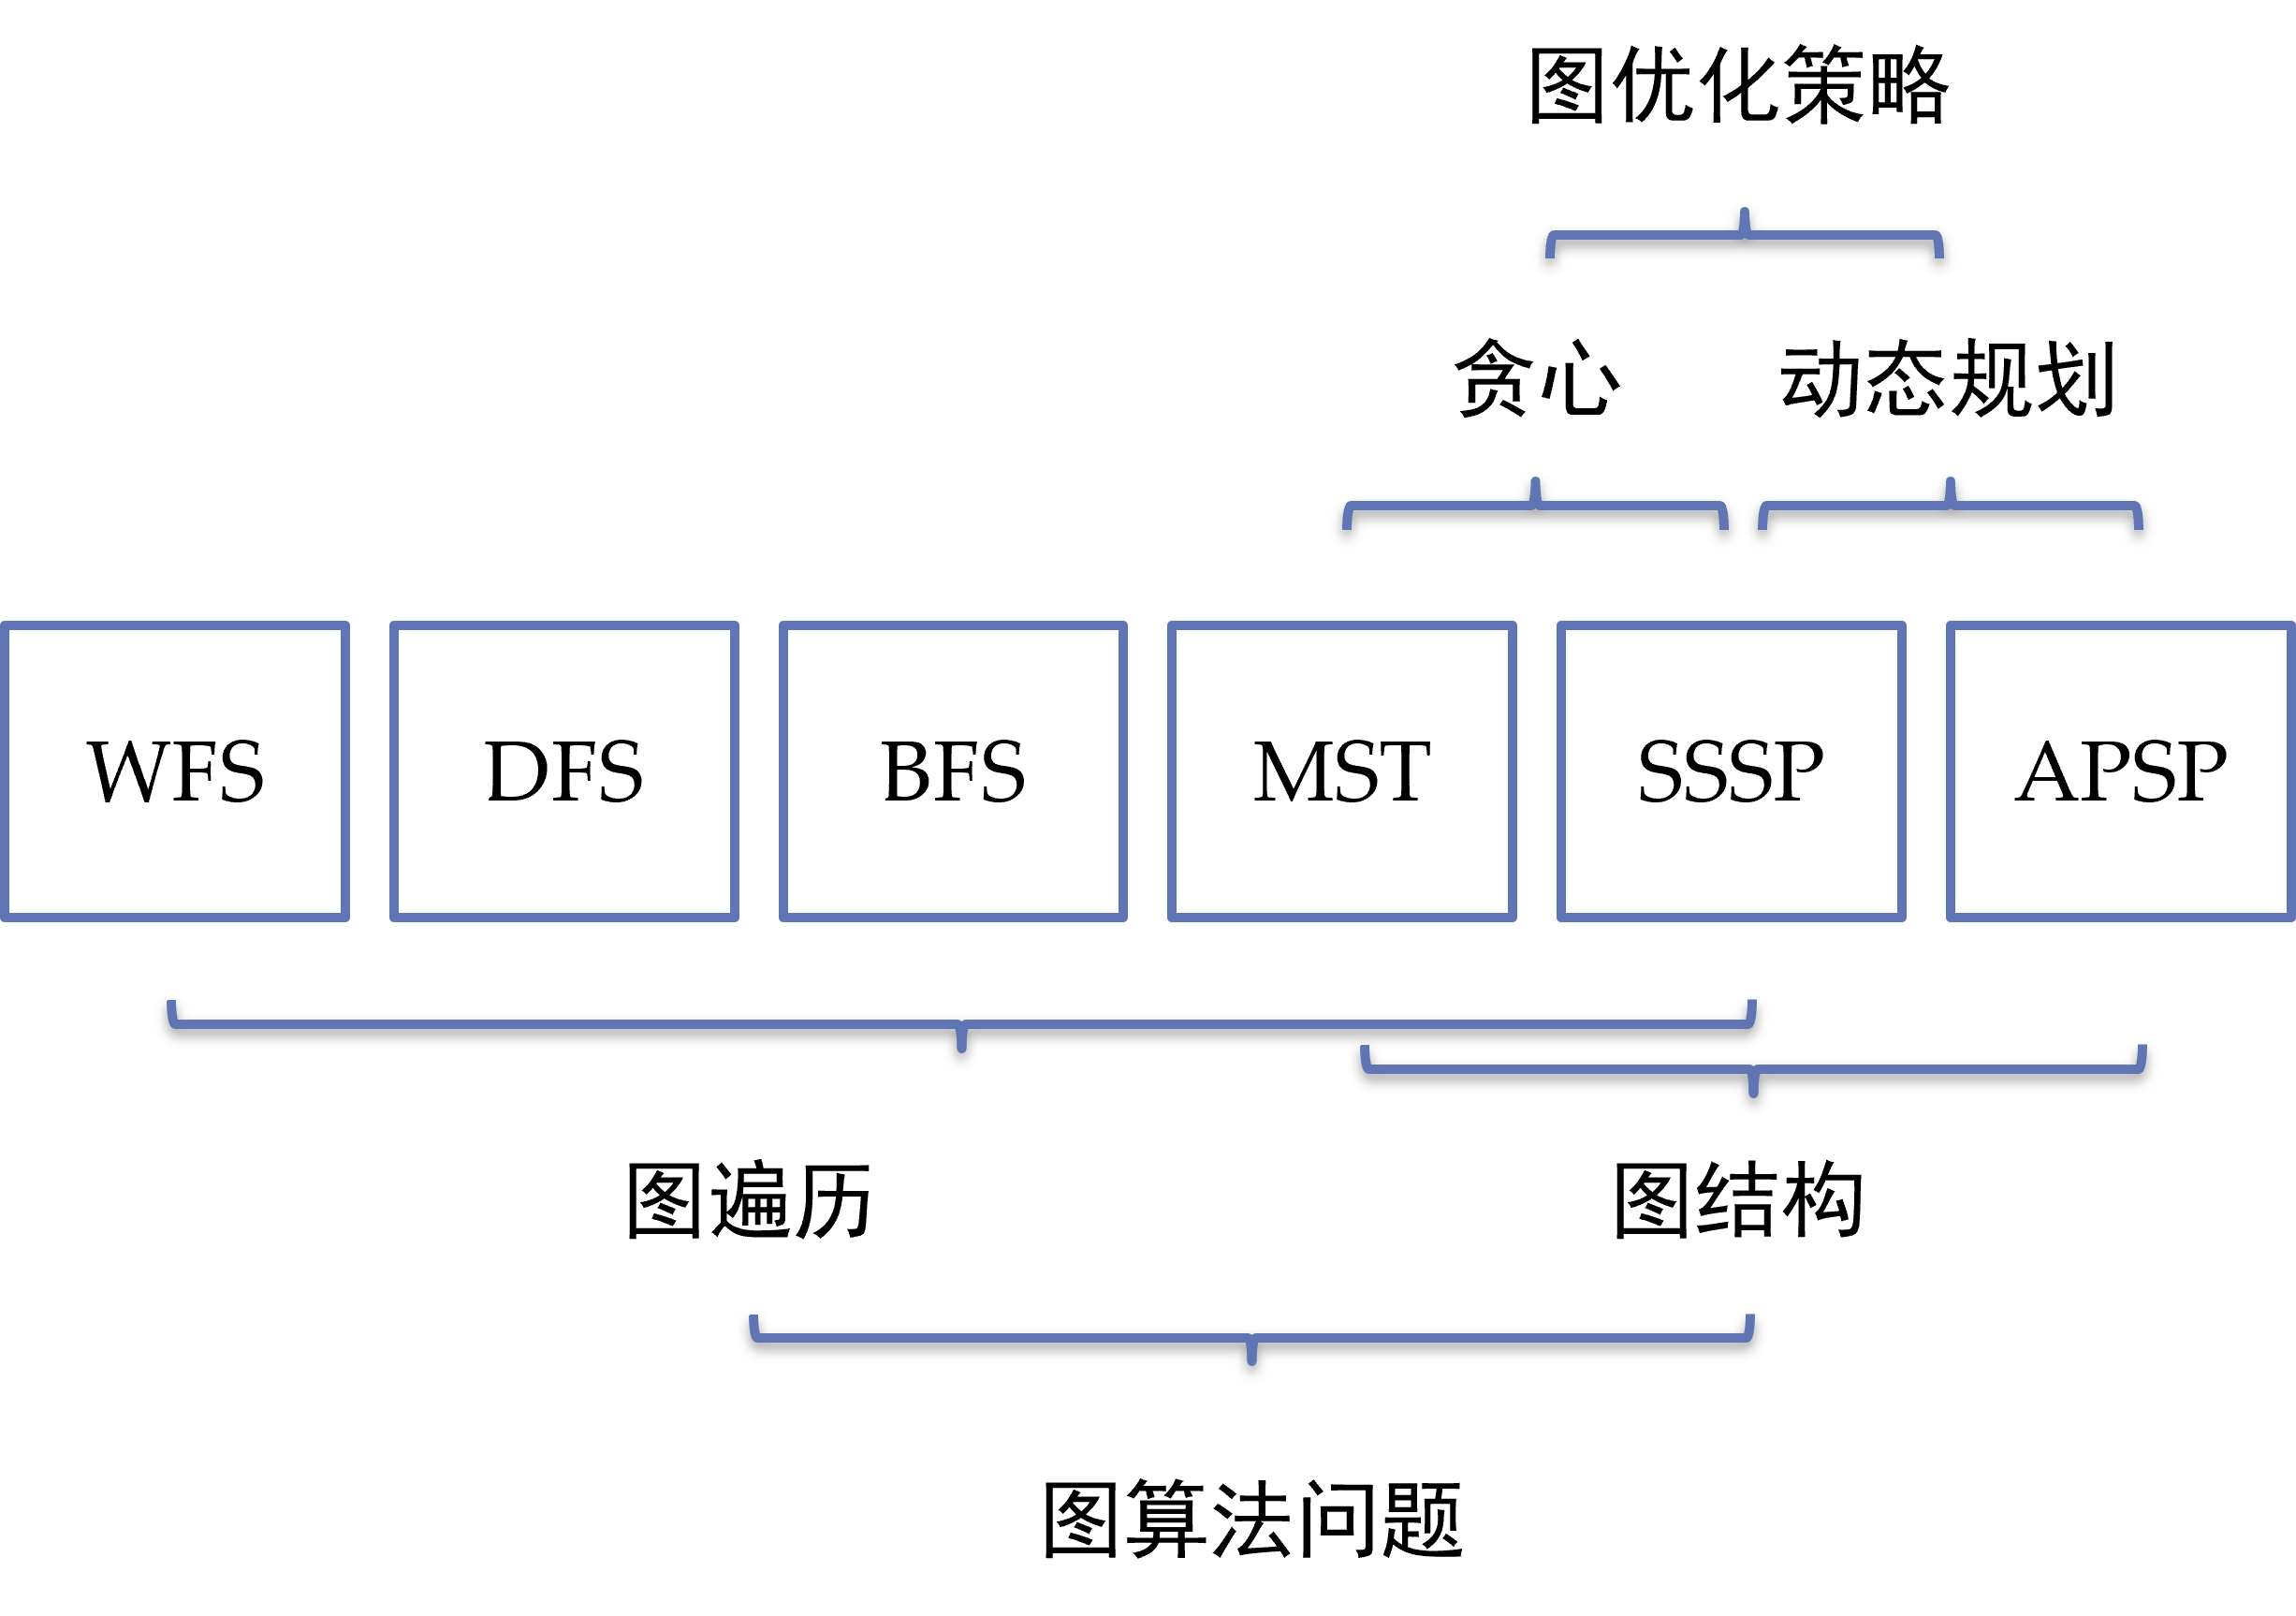
\includegraphics[width=0.6\columnwidth]{./figs/graph-trav/overview.png}
    \caption{图算法知识点总览}
    \label{fig:graph-overview}
\end{figure}

%----------------------------------------
\section{WFS遍历框架} \label{sec:wfs}

\nid “爱谁谁优先遍历”\alg{WhateverFirstSearch}（WFS）：
%--
\begin{itemize}
    \item 基本做法：从一个点，顺着边，走到下一个点，直至走遍所有点和边。
    \item 设计要点：
    %--
    \begin{itemize}
        \item 调度：抽象的bag结构（具体设计由后续的设计者来决定）；
        \item 去重：点的二着色。
    \end{itemize}
\end{itemize}

%--------------------
\subsection{WFS的设计}

WFS的设计，如算法\ref{alg:wfs}所示。
WFS的外层调用过程（wrapper）的设计，如算法\ref{alg:wfs-wrapper}所示。

%--
\begin{algorithm}[htbp]
    \caption{WFS($s$)}
    \label{alg:wfs}
    \begin{algorithmic}[1]
        \State put $s$ into the bag $B$
        \While{$B$ is not empty}
        \State take $v$ from $B$
        \If{$v$ is unmarked}
        \State mark $v$
        \ForAll{edge $vw$}
        \State put $w$ into $B$
        \EndFor
        \EndIf
        \EndWhile
    \end{algorithmic}
\end{algorithm}


%--
\begin{algorithm}[htbp]
    \caption{\alg{WFSWrapper}($G$)}
    \label{alg:wfs-wrapper}
    \begin{algorithmic}[1]
        \ForAll{vertices $v$}
        unmark $v$ \Comment{遍历之前，初始化每个点}
        \EndFor
        \ForAll{vertices $v$}
        \If{$v$ is unmarked}
        WFS($v$)
        \EndIf
        \EndFor
    \end{algorithmic}
\end{algorithm}

%--------------------
\subsection{从WFS逐步精化}

以支撑遍历过程的“枢纽”性的数据结构为抓手，我们可以统一各类“遍历”算法，如图\ref{fig:wfs}所示。

%--
\begin{figure}[htbp]
    \center
    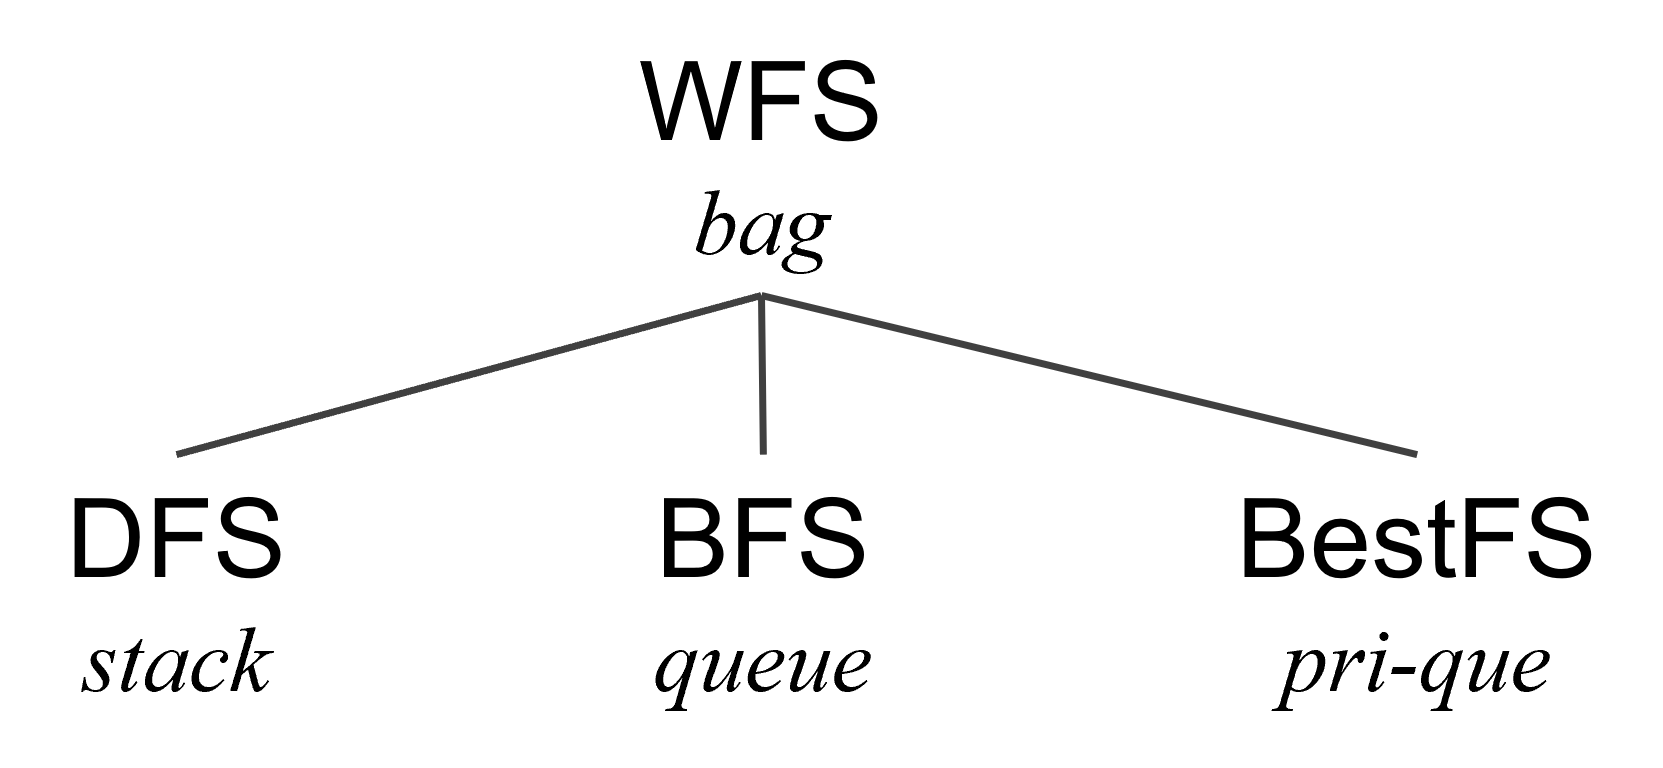
\includegraphics[width=0.5\columnwidth]{./figs/graph-trav/wfs.png}
    \caption{WFS框架的精化}
    \label{fig:wfs}
\end{figure}

